\chapter{Dasar Teori}
\label{chap:dasar_teori}
	
\section{Kecerdasan Bisnis}
\label{sec:kecerdasan_bisnis}
Kecerdasan bisnis dapat diartikan sebagai suatu kumpulan metode, proses, teori, arsitektur dan teknologi yang dapat mengubah data menjadi informasi yang bermanfaat dan memiliki nilai yang berguna dalam kepentingan bisnis. Sistem kecerdasan bisnis dapat menyediakan data di masa lalu dan saat ini. Data yang ditampilkan dapat berupa laporan, statistik, dll. Selain itu data data yang ditampilkan dapat dilihat berdasarkan suatu dimensi tertentu, misal berdasarkan dimensi waktu, pelanggan, dll.

\section{Integrasi Sistem Kecerdasan Bisnis dalam Sistem Big Data}
\label{sec:integrasi_kecerdasan_bisnis}

\section{Sosial Media Twitter}
\label{sec:twitter}
Twitter adalah sebuah situs web yang dimiliki dan dioperasikan oleh Twitter Inc.. Twitter menawarkan jaringan sosial mikroblog dengan panjang pesan maksimal hingga 140 karakter, yang biasanya disebut Tweet. Melalui mikroblog Twitter, pengguna dapat memperbarui status terbaru tentang hal yang sedang mereka pikirkan ataupun berpendapat tentang suatu objek atau fenomena tertentu. Pesan yang dibuat pengguna akan tampil secara langsung dan dapat dilihat seluruh dunia melalui website Twitter atau berbagai aplikasi eksternal lainnya. Untuk menghemat karakter pada sebuah tweet biasanya pengguna menuliskan singkatan, bahasa slang atau emoticon dalam mengkomunikasikan pesannya. 

Pengguna Twitter dapat mengelompokan tweetnya dengan menggunakan hastags - kata atau frasa yang diawali dengan tanda "\#". Selain itu pengguna juga dapat menunjuk pengguna lainnya dengan menuliskan username mereka diawali dengan tanda "@". Setiap tweet yang dibuat dapat dibalas ataupun di tweet ulang (re-tweet) oleh pengguna lainnya.

\subsection{Twitter Streaming API}
\label{sec:twitter_streaming_api}
Twitter menyediakan Streaming API yang memudahkan pengembang aplikasi untuk mendapatkan tweet-tweet yang dibuat pengguna Twitter secara realtime. Streaming API yang tersedia memiliki beberapa jenis sesuai dengan kegunaannya, yaitu:

\begin{enumerate}
	\item \textbf{Public Streams}: Untuk melakukan streaming pada data publik secara realtime. Cocok untuk digunakan pada pencarian tweet berdasarkan user atau topik tertentu dan data mining.
	\item \textbf{User Streams}: Untuk melakukan streaming pada single-user, hasil streaming terdiri dari data-data yang berkaitan dengan kegiatan single-user.
	\item	\textbf{Site Streams}: Merupakan versi multi-user dari User Streams. Site Streams dimaksudkan untuk server yang harus terhubung ke Twitter atas nama banyak pengguna.
\end{enumerate}

\begin{figure}
\centering
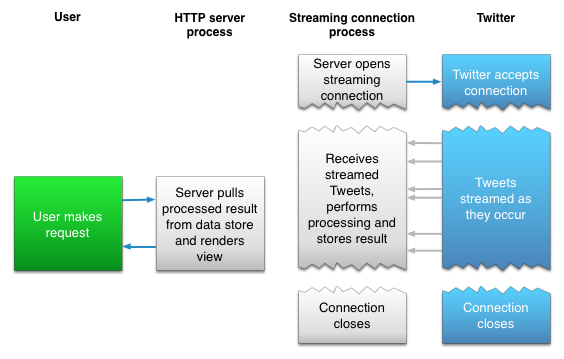
\includegraphics[scale=0.5]{Gambar/streaming-intro-2_1.png}
\caption[Proses Twitter Streaming API]{Proses Twitter Streaming API \cite{TwitterApi:2015}} 
\end{figure}

\section{Data Mining}
\label{sec:data_mining}
\subsection{Pengertian Data Mining}
Saat ini pertumbuhan informasi berkembang sangat cepat setiap harinya. Jutaan bahkan milyaran data dari proses bisnis, sosial, sains, dan hampir setiap aspek kehidupan kita dituangkan ke dalam berbagai perangkat penyimpanan data. Pertumbuhan data yang pesat dan penyimpanan dalam basis data yang besar dan banyak telah melampaui kemampuan manusia dalam memahami isi dari data tertsebut. Oleh karena itu data mining sangat diperlukan dalam menggali informasi atau pola yang terdapat di dalam tumpukan data yang sangat besar. Data-data yang akan ditambang dapat berasal dari basis data relasional, data warehouse, transactional database, advanced database system, flat file, data stream, text or multimedia. \cite{han2011data} 

\subsection{Proses \textit{Knowledge Discovery}}
Proses \textit{Knowledge Discovery} adalah proses pencarian pengetahuan pada data dapat berupa informasi atau pola. Dalam proses \textit{Knowledge Discovery} perlu dilakukan langkah-langkah seperti berikut.

\begin{enumerate}
	\item Data cleaning \\Proses pembersihan data yang kotor dan tidak konsisten.
	\item Data integration \\Proses untuk menyatukan data-data dari berbagai sumber lainnya.
	\item Data selection \\Proses pemilihan data yang relevan dengan analisis yang diambil dari basis data.
	\item Data transformation \\Proses perubahan data ke dalam bentuk yang sesuai untuk proses penambangan dengan melakukan ringkasan atau agregasi operasi.
	\item Data mining \\Proses dimana metode-metode diterapkan untuk mendapatkan informasi atau pola yang berguna.
	\item Pattern evaluation \\Proses melakukan evaluasi pada pola atau informasi yang diperoleh.
	\item Knowledge presentation \\Proses memvisualisasi pola atau informasi yang digunakan untuk menyajikan hasil penambangan kepada pengguna.
\end{enumerate}


\begin{figure}
\centering
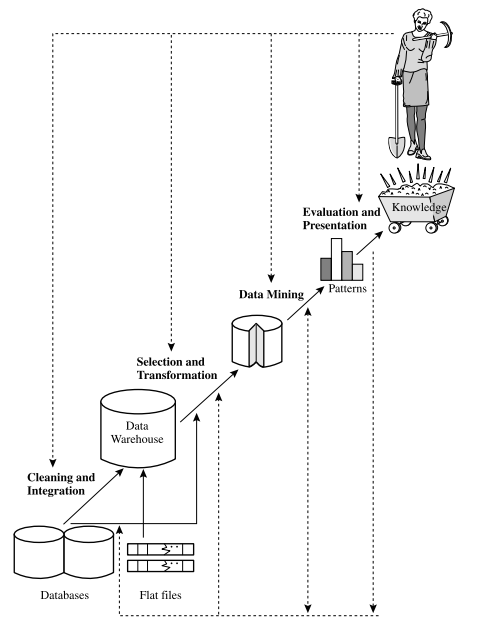
\includegraphics[scale=0.5]{Gambar/data-mini-process.png}
\caption[Step dalam melakukan Proses \textit{Knowledge Discovery}]{Step dalam melakukan Proses \textit{Knowledge Discovery} \cite{han2011data}} 
\end{figure}


\subsection{Teknik-Teknik Data Mining}
\begin{enumerate}
	\item \textit{Classification} (Pengklasifikasian)
	\textit{Classification} adalah proses menemukan fitur-fitur yang sama pada sebuah himpunan data di dalam basis data dan mengklasifikasikannya ke dalam kelas-kelas sesuai model klasifikasi yang ditetapkan. Proses \textit{Classification} terdiri dari dua langkah yaitu langkah pembelajaran (model klasifikasi dibangun) dan langkah klasifikasi (model digunakan untuk memprediksi kelas untuk data yang diberikan). Classification dikenal pula sebagai supervised learning di mana kelas-kelas telah didefinisikan sebelumnya.
	\item \textit{Clustering} (Pengelompokan)
	\textit{Clustering} adalah proses pengelompokan satu set benda-benda ke dalam kelas objek yang sama. Sebuah \textit{Cluster} adalah kumpulan objek data yang mirip satu sama lain dalam Cluster yang sama dan berbeda dengan benda-benda di cluster lain. Clustering dikenal juga sebagai unsupervised learning dimana kelas-kelas tidak diketahui sebelumnya. Clustering juga disebut segmentasi data dalam beberapa aplikasi karena mengelompokkan data set yang besar menjadi kelompok-kelompok yang memiliki kesamaan. 
	\item \textit{Regression} (Regresi)
	Regression hampir mirip dengan pengklasifikasian. Akan tetapi, Regression menggunakan nilai yang ada untuk memperkirakan nilai yang akan muncul kemudian. Cara untuk mengetahui ketepatan dari pengklasifikasian adalah dengan menggunakan \textit{wait} and \textit{see}.
\end{enumerate}

\section{Text Mining}
\label{sec:text_mining}

\subsection{Pengertian Text Mining}
Text mining adalah salah satu bidang khusus dari data mining. Text mining dapat didefinisikan sebagai suatu proses menggali informasi dimana seorang user berinteraksi dengan sekumpulan text menggunakan tools analisis yang merupakan komponen-komponen dalam data mining yang salah satunya adalah kategorisasi. \cite{feldman2006j} Tujuan dari text mining adalah untuk mendapatkan informasi yang berguna dari sekumpulan text. Sumber data yang digunakan pada text mining adalah kumpulan text yang memiliki format yang tidak terstruktur atau minimal semi terstruktur. Adapun tugas khusus dari text mining antara lain yaitu pengkategorisasian text (\textit{text categorization}) dan pengelompokan text (\textit{text clustering}).

Permasalahan yang dihadapi pada text mining sama dengan permasalahan yang terdapat pada data mining, yaitu jumlah data yang besar, dimensi yang tinggi, data dan struktur yang terus berubah, dan data \textit{noise}. Perbedaan di antara keduanya adalah pada data yang digunakan. Pada data mining, data yang digunakan adalah data terstruktur, sedangkan pada text mining, data yang digunakan pada umumnya adalah data tidak terstruktur atau minimal semiterstruktur. Hal ini menyebabkan adanya tantangan tambahan pada text mining yaitu struktur text yang kompleks dan tidak lengkap, arti yang tidak jelas serta tidak umum, dan bahasa yang berbeda-beda.

\subsection{Proses Text Mining}
\begin{figure}
\centering
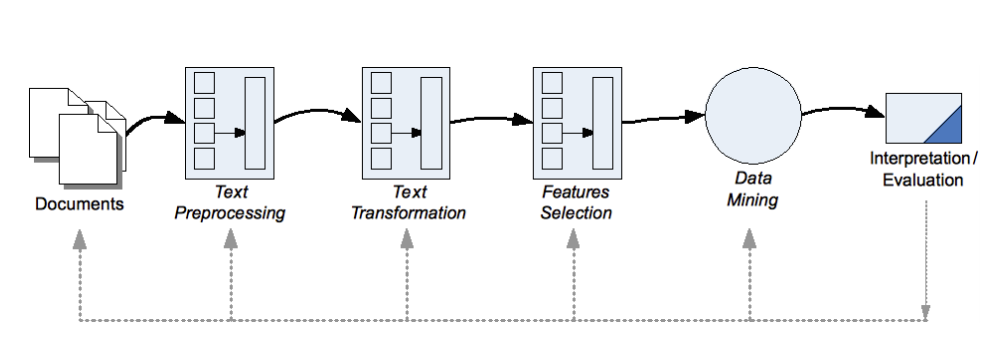
\includegraphics[scale=0.5]{Gambar/proses-text-mining.png}
\caption[Proses Text Mining]{Proses Text Mining.\\Sumber: http://lecturer.ukdw.ac.id/budsus/pdf/textwebmining/TextMining\_Kuliah.pdf} 
\end{figure}

Proses-proses yang umumnya dilakukan dalam melakukan Text Mining adalah

\begin{enumerate}
	\item Text Preprocessing\\
	Tahap text preprocessing adalah tahap awal dari text mining. Tahap ini mencakup semua rutinitas, dan proses untuk mempersiapkan data yang akan digunakan pada operasi \textit{knowledge discovery} sistem text mining. \cite{feldman2007text}. Biasanya pada proses ini text akan diubah ke dalam huruf kecil lalu terjadi pembuangan delimiter-delimiter seperti tanda baca.
	
	\item Text Transformation\\
	Pada tahap ini teks akan diubah bentuknya sesuai dengan kebutuhan proses penambangan.
	
	\item Feature Selection\\
	Tahap seleksi fitur (feature selection) bertujuan untuk mengurangi dimensi dari suatu kumpulan teks, atau dengan kata lain menghapus kata-kata yang dianggap tidak penting atau tidak menggambarkan isi dokumen sehingga proses pengklasifikasian lebih efektif dan akurat. \cite{manalu2014analisis}. Pada tahap ini tindakan yang dilakukan adalah menghilangkan \textit{stopword} (\textit{stopword removal}) dan \textit{stemming} terhadap kata yang berimbuhan.\cite{berry2010text}
	
	\textit{Stopword} adalah kosakata yang bukan merupakan ciri dari suatu teks. Misalnya "di", "oleh", "pada", "selama", "sebab" dan lain sebagainya. Sebelum proses \textit{stopword removal} dilakukan, harus dibuat daftar stopword (stoplist). Jika termasuk di dalam stoplist maka kata-kata tersebut akan dihapus dari deskripsi sehingga kata-kata yang tersisa di dalam deskripsi dianggap sebagai kata-kata yang mencirikan isi dari suatu dokumen atau keywords. Daftar kata stopword di penelitian ini bersumber dari Tala (2003) \cite{tala2003study}.
	
	Setelah melalui proses \textit{stopword removal} langkah berikutnya adalah proses \textit{stemming}. \textit{Stemming} adalah proses pemetaan dan penguraian berbagai bentuk (variants) dari suatu kata menjadi bentuk kata dasarnya (stem) \cite{tala2003study}. Tujuan dari proses ini adalah untuk menghilangkan imbuhan-imbuhan baik itu berupa prefiks, sufiks, maupun konfiks yang ada pada setiap kata. \cite{manalu2014analisis} Dengan adanya proses stemming ini maka dimensi data akan berkurang sehingga data dapat diproses dengan lebih cepat dan akurat.
\end{enumerate}


\section{Sentimen Analisis}
\label{sec:sentimen_analisis}
Sentimen analisis mengacu pada bidang yang luas dari pengolahan bahasa alami, komputasi linguistik dan text mining yang bertujuan menganalisis pendapat, sentimen, evaluasi, sikap, penilaian dan emosi seseorang apakah pembicara atau penulis berkenaan dengan suatu topik, produk, layanan, organisasi, individu, ataupun kegiatan tertentu. \cite{liu2012sentiment} Hasil dari sentimen analisis berupa kelompok teks dengan nilai sentimen positif, netral atau negatif pada suatu objek tertentu.

\section{Hadoop}
\label{sec:hadoop}

\subsection{Pengertian Hadoop}
\label{sec:pengertian_hadoop}
Apache Hadoop adalah sebuah framework opensource yang memungkinkan untuk memproses set data yang besar secara terdistribusi di cluster komputer menggunakan model pemrograman yang sederhana. Hadoop dirancang untuk meningkatkan kemampuan server tunggal menjadi ribuan mesin yang masing-masing menawarkan komputasi dan penyimpanan lokal. Hadoop sendiri dirancang untuk mendetexti dan menangani kegagalan pada lapisan aplikasi, sehingga memberikan layanan yang \textit{highly-available} pada sekelompok komputer yang masing-masingnya mungkin rentan terhadap kegagalan. Hal tersebut lebih baik dibanding hanya mengandalkan perangkat keras untuk memberikan \textit{high-availability}.

\subsection{Komponen Utama Hadoop}
\label{sec:komponen_utama_hadoop}
Hadoop pada dasarnya memiliki empat buah komponen utama, yaitu:
\begin{enumerate}
	\item Hadoop Common\\
	Hadoop Common adalah utilitas umum yang mendukung modul lain di Hadoop.
	\item Hadoop Distributed File System (HDFS)\\
	HDFS adalah sebuah file sistem yang didesain untuk memproses data distribusi skala besar di dalam framwork seperti MapReduce. HDFS dapat menyimpan sebuat data set sebesar 100TB sebagai sebuah single file.\cite{Lam:2010:HA:1965594} HDFS bisa bersifat single node atau multiple node. HDFS bukan native File System seperti layaknya EXT3, EXT4, FAT atau NTFS. HDFS ada pada layer di atasnya.
	
	\item Hadoop YARN\\
	Hadoop YARN atau Yet Another Resource Negotiator adalah teknologi untuk mengatur \textit{resource} dan \textit{scheduling} pada sebuah cluster.
	\item Hadoop MapReduce\\
	MapReduce adalah sebuah model pemrosesan data\cite{Lam:2010:HA:1965594}. MapReduce ditujukan untuk memproses data berukuran raksasa secara terdistribusi dan paralel dalam cluster yang terdiri atas banyak komputer. Dalam memproses data, secara garis besar MapReduce dapat dibagi dalam dua proses yaitu proses \textit{Map} dan proses \textit{Reduce}. Kedua jenis proses ini didistribusikan ke setiap komputer nodes dalam suatu cluster (kelompok komputer yang salih terhubung) dan berjalan secara paralel tanpa saling bergantung satu dengan yang lainnya. Proses \textit{Map} bertugas untuk mengumpulkan informasi dari potongan-potongan data yang terdistribusi dalam tiap komputer dalam cluster. Hasilnya diserahkan kepada proses \textit{Reduce} untuk diproses lebih lanjut. Hasil proses Reduce merupakan hasil akhir yang dikirim ke pengguna. \cite{Dean:2008:MSD:1327452.1327492}
	
	\begin{figure}
		\centering
		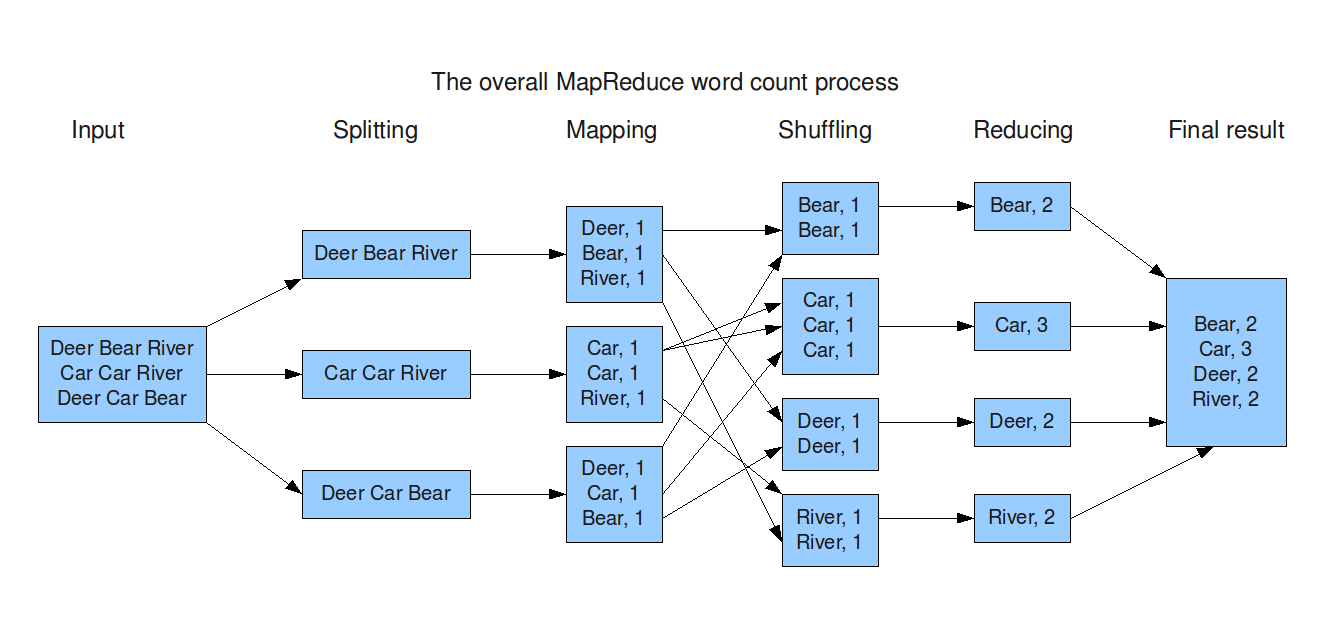
\includegraphics[scale=0.4]{Gambar/MapReduce_Work_Structure.png}
		\caption[Contoh Cara Kerja MapReduce]{Contoh Cara Kerja MapReduce. \\Sumber: http://www.milanor.net/blog/?p=853}
	\end{figure}
	
\end{enumerate}

\subsection{Sqoop}
\label{sec:sqoop}
Apache Sqoop adalah sebuah \textit{tool} yang dirancang untuk mentransfer data dari Apache Hadoop ke tempat penyimpanan data terstruktur seperti basis data relasional secara efisien. Sqoop dapat dimanfaatkan untuk menyimpan informasi atau pola yang dihasilkan dari proses text mining ke dalam sistem kecerdasan bisnis. \cite{sqoop:2015}

\subsection{Hive}
\label{sec:hive}
Apache Hive adalah perangkat lunak \textit{data warehouse} yang memfasilitasi kueri dan mengelola dataset besar yang berada dalam penyimpanan terdistribusikan. Dibangun di atas Apache Hadoop, ia menyediakan hal-hal berikut ini.\cite{hive:2015}

\begin{itemize}
	\item \textit{Tools} yang memudahkan proses data extract/transform/load (ETL)
	\item Suatu mekanisme untuk menentukan struktur pada berbagai format data
	\item Akses ke file yang tersimpan baik secara langsung di Apache HDFS atau dalam sistem penyimpanan data lainnya seperti Apache HBase
	\item Eksekusi kueri melalui MapReduce
\end{itemize}

Hive mendefinisikan sebuah SQL sederhana seperti bahasa kueri yang disebut QL. QL memungkingkan pengguna yang terbiasa dengan SQL untuk melakukan kueri pada data. Bahasa ini juga memungkinkan programmer yang terbiasa dengan MapReduce untuk menyambungkan \textit{custom mapper} dan \textit{reducer} untuk melakukan analisis yang lebih canggih yang mungkin tidak didukung oleh kemampuan \textit{built-in} bahasa pemrogramman. QL juga memiliki \textit{custom scalar functions} (UDF's), \textit{aggregations} (UDAF's), dan \textit{table functions} (UDTF's). \cite{sqoop:2015}